%%%%%%%%%%%%%%%%%%%%%%% file template.tex %%%%%%%%%%%%%%%%%%%%%%%%%
%
% This is a general template file for the LaTeX package SVJour3
% for Springer journals.          Springer Heidelberg 2010/09/16
%
% Copy it to a new file with a new name and use it as the basis
% for your article. Delete % signs as needed.
%
% This template includes a few options for different layouts and
% content for various journals. Please consult a previous issue of
% your journal as needed.
%
%%%%%%%%%%%%%%%%%%%%%%%%%%%%%%%%%%%%%%%%%%%%%%%%%%%%%%%%%%%%%%%%%%%
%
% First comes an example EPS file -- just ignore it and
% proceed on the \documentclass line
% your LaTeX will extract the file if required
%\begin{filecontents*}{example.eps}
%%!PS-Adobe-3.0 EPSF-3.0
%%%BoundingBox: 19 19 221 221
%%%CreationDate: Mon Sep 29 1997
%%%Creator: programmed by hand (JK)
%%%EndComments
%gsave
%newpath
%  20 20 moveto
%  20 220 lineto
%  220 220 lineto
%  220 20 lineto
%closepath
%2 setlinewidth
%gsave
%  .4 setgray fill
%grestore
%stroke
%grestore
%\end{filecontents*}
%
\RequirePackage{fix-cm}
%
%\documentclass{svjour3}                     % onecolumn (standard format)
%\documentclass[smallcondensed]{svjour3}     % onecolumn (ditto)
%\documentclass[smallextended]{svjour3}       % onecolumn (second format)
\documentclass[twocolumn]{svjour3}          % twocolumn
%
\smartqed  % flush right qed marks, e.g. at end of proof
%
\usepackage{graphicx}
\usepackage{amssymb}
\usepackage{graphicx}
\usepackage{amsmath,amssymb,latexsym,float,epsfig,subfigure}
\usepackage{mathtools, bbm}
\usepackage{amsmath} % assumes amsmath package installed
\usepackage{amssymb}  % assumes amsmath package installed
\usepackage{lipsum}
\usepackage[export]{adjustbox}
\usepackage[normalem]{ulem} % underline
\usepackage{wrapfig}
\usepackage{multirow}
\usepackage{balance}
\usepackage{color}
\usepackage{url}
\usepackage[breaklinks=true]{hyperref}
\usepackage{breakcites}
\usepackage{microtype}
\usepackage{natbib}
\usepackage{algorithm, algorithmic}
\def\bibfont{\footnotesize}
\newcommand{\norm}[1]{\left\lVert#1\right\rVert}

%
% \usepackage{mathptmx}      % use Times fonts if available on your TeX system
%
% insert here the call for the packages your document requires
%\usepackage{latexsym}
% etc.
%
% please place your own definitions here and don't use \def but
% \newcommand{}{}
%
% Insert the name of "your journal" with
 \journalname{Autonomous Robots}
%
\begin{document}

\title{Working title%\thanks{Grants or other notes
%about the article that should go on the front page should be
%placed here. General acknowledgments should be placed at the end of the article.}
}
\subtitle{Humans helping robots helping humans}

%\titlerunning{Short form of title}        % if too long for running head

\author{Deepak E. Gopinath$^*$      \and
        Brenna D. Argall %etc.
}

%\authorrunning{Short form of author list} % if too long for running head

\institute{ Deepak Gopinath \at
            Department of Mechanical Engineering\\
            Northwestern University, Evanston, IL\\
              Tel.: +123-45-678910\\
              Fax: +123-45-678910\\
              \email{deepakgopinath@u.northwestern.edu}           %  \\
%             \emph{Present address:} of F. Author  %  if needed
           \and
           Brenna Argall \at
}

\date{Received: date / Accepted: date}
% The correct dates will be entered by the editor


\maketitle

\begin{abstract}
Assistive human cyber-physical systems have the potential to transform the lives of millions of people afflicted with severe motor impairments as a result of spinal cord or brain injuries. The effectiveness and usefulness of assistive systems, however, is closely related to their ability to infer the user's needs and intentions and is often a limiting factor for providing appropriate assistance \textit{quickly, confidently and accurately}. The contributions of this paper are two-fold: firstly, we leverage the notion of \textit{inverse legibility} and propose a goal disambiguation algorithm which enhances the intent inference and assistive capabilities of a shared-control assistive robotic arm. Secondly, we introduce a novel intent inference algorithm that works in conjunction with the disambiguation scheme, inspired by dynamic field theory in which the time evolution of the probability distribution over goals is specified as a dynamical system. We also present a experimental study to evaluate the efficacy of the disambiguation system. This study was performed with ten subjects. Results show that upon operating the robot in the control mode picked by the disambiguation algorithm, the progress towards the goal significantly became faster as a result of accurate and confident robot assistance and the number and rate of mode switches performed by the user decreased as well. 
\keywords{Shared Autonomy \and Intent Inference \and Intent Disambiguation \and Assistive Robotics}
% \PACS{PACS code1 \and PACS code2 \and more}
% \subclass{MSC code1 \and MSC code2 \and more}
\end{abstract}

\section{Introduction}\label{sec:intro}
%Assistive Robotics and what it can do

Assistive and rehabilitation machines---such as assitive robotic arms and powered wheelchairs---have the potential to transform the lives of millions of people with severe motor impairments~\cite{laplante1992assistive}. These devices can promote independence, boost self-esteem and help to extend the mobility and manipulation capabilities of such individuals, thereby revolutionizing the way motor-impaired people interact with society~\cite{scherer1996outcomes, huete2012personal}. With the rapid technological strides in the domain of assistive robotics, the devices have become more capable and complex---to the extent that control of these devices becomes a greater challenge. 

The control of an assistive device is typically facilitated via a control interface. The greater the motor impairment of the user, the more limited are the interfaces available for them to use. These interfaces (for example, Sip-N-Puff and switch-based head arrays) are low dimensional, discrete interfaces that can operate only in subsets of the entire control space~\cite{simpson2008tooth, nuttin2002selection}. 
The dimensionality mismatch between the control interfaces and the controllable degrees-of-freedom of the assistive robot necessitates the partitioning of the entire control space into smaller subsets called \textit{control modes}. In order to achieve full control of the robot, the user switches between the control modes and this is referred to as \textit{mode switching} or \textit{modal control}~\cite{herlant2016assistive}. More importantly, when the control interface is more limited and low-dimensional, the greater number of control modes there are. 

Mode switching adds to the cognitive and physical burden during task execution and has a detrimental effect on the performance~\cite{eftring1999technical}. The introduction of \textit{shared robotics autonomy} to these assistive cyber-physical systems seeks to alleviate some of these issues. The task responsibility is shared between the user and the robot thereby reducing the human effort in achieving a goal. Shared autonomous systems arbitrate between the human control commands and the robot autonomy using different strategies depending on the task context, user preferences and robotic platform. Figure 1 depicts the most important components of a  typical shared control architecture.

As depicted in Figure 1, any assistive robotic system needs to have a good idea of what the user's needs and intentions are. That is, intent inference is a necessary and crucial component to ensure appropriate assistance. Even in the context of human-human teams, mutual action understanding happens in an online fashion during the time course of interaction and makes collaborative task execution more seamless and efficient. The notion of shared intentionality, one in which all parties involved in a collaborative task team share the same intention is shown to improve task performance significantly (rephrase, cite). This principle is also relevant and important in the context of human-robot interaction. Specifically, in assistive robotic manipulation, since the robotic device is primarily used for reaching toward and grasping of discrete objects in the environment, intent inference can be framed as a problem of estimating the probability distribution over all possible goals (objects) in the environment. This inference is usually informed by various cues from the human and the environment such as the control actions issued by the human, features relevant to the robot and goal locations and biometric measures that indicate the cognitive and physical load of the user during task execution. More the number of cues available it is likely that the inference becomes more accurate. 

However, in the assistive domain user satisfaction and comfort is of paramount importance for the acceptance and adoption of these technologies. Adding more sensors to track biometric data and objects locations become expensive and cumbersome and can likely affect the user experience in a negative way. Therefore, in our work, we rely primarily on the user control command issued via the control interface to inform the inference. This in turn, makes the inference problem harder for the robot and necessitates the need for robust intent inference formalisms. 

Our key insight is that we have a human in the loop and certain control commands issued by the human may contain more information and are \textit{more intent expressive} and \textit{legible} which can likely help the robot draw useful and more accurate inferences. This is the notion of \textit{inverse legibility} in which human-generated actions \textit{help the robot} to infer the human's intent unambiguously. Consider the hypothetical reaching experiment illustrated in Figure 2. Since the spatial locations of the goal are maximally spread along the horizontal axis, any human control command issued along the $x$ dimension conveys the intended goal unequivocally to the robot. Or in other words, it is more \textit{intent expressive} and will help the robot to draw accurate inference more quickly and confidently. This approach to more seamless human-robot interaction exploits the underlying synergies and symbiotic relationship that is inherent in task execution with a shared intention. 

In this work, as our primary contribution we develop a mode switch assistance paradigm that helps the robot with intent inference, by selecting the control mode in which a user-initiated motion will \textit{maximally disambiguate} human intent. The intent disambiguation layer sits atop a given intent inference mechanism as depicted in Figure 1. Consequently, the disambiguation power of the algorithm is closely linked to and is dependent on the success and accuracy of the underlying intent inference mechanism. More specifically on how well past cues are incorporated into the inference process. As our secondary contribution, we develop a novel intent inference scheme that efficiently incorporates information contained in past cues thereby ensuring the success of the disambiguation paradigm. 

In Section~\ref{sec:related-work} we present a comprehensive overview of relevant research in the area of shared autonomy is assistive robotics, types of assistive paradigms, intent inference and synergies in human-robot interaction. Section~\ref{sec:ma} presents the mathematical formalism developed for intent inference and disambiguation and Section~\ref{sec:implementation} focuses on the implementation details. The study design and experimental methods are discussed in Section~\ref{sec:ed} followed by results in Section~\ref{sec:results}. Discussions and conclusions are presented in Sections~\ref{sec:discussions} and~\ref{sec:conclusions} respectively. 


%%Understanding intent is critical. Why? Shared intention in human-human teams. Human-robot teams. Different types of paradigms exist for the same. 
%
%But we have human-in-th-loop. If the robot can elicit more intent expressive actions from the user, the inference problem becomes easier for the robot. Therefore the intent disambiguation system. 


\section{Related Work}\label{sec:related-work}
This section provides a comprehensive overview of related research in the domains of shared autonomy in assistive robotics, robot assistance for modal control, intent inference in human-robot interaction and information acquisition in robotics. 

Shared-autonomy in assistive systems aims to reduce user's cognitive and physical burden during task execution without having the user relinquish complete control~\cite{philips2007adaptive,demeester2008user, gopinath2017human, muelling2017autonomy}. Shared autonomy is preferred over fully autonomous robotic systems due to enhanced user satisfaction and robustness. The most common strategies to share control between the user and the assistive system include a) a hierarchical paradigm in which the higher level goals are entrusted with the user and the autonomy generates low-level control~\cite{tsui2011want, kim2010relationship, kim2012autonomy}, b) control allocation in distinct partitions of the entire control space~\cite{driessen2005collaborative} and c) blending user controls and robot autonomy commands~\cite{downey2016blending, storms2014blending, muelling2017autonomy}. 

In order to offset the drop in task performance due to shifting focus (\text{task switching}) from the task at hand to switching between different control modes different mode switch assistance paradigms have been proposed. Even a simple time-optimal mode switching scheme has shown to improve task performance~\cite{herlant2016assistive}. Mode switch assistance schemes have also been proposed as a goal disambiguation mechanism which will help in improving the robot's intent inference capabilities~\cite{gopinath2017mode}. 

Shared control system often requires a good estimate of the humans' intent---for example, their intended reach target in a manipulation task or a target location in the environment in navigation task~\cite{liu2016goal}. Intent can either be explicitly communicated by the user~\cite{choi2008laser} or can be inferred using various algorithms from their control signals or sensor data. Intent recognition and inference is an actively studied by cognitive scientists and roboticists and can be broadly categorized into two main classes: model-based approaches and heuristic approaches. In the model-based approach, intent inference is typically cast within the Bayesian framework and the posterior distribution over goals at any time is determined by the iterative application of Bayes theorem. Evidence in this context can be derived from a combination of various factors such as environmental cues, control commands, biometric data from the user \textit{et cetera}~\cite{baker2007goal, baker2009action}. The user is modeled as a Partially Observable Markov Decision Process (POMDP) and is assumed to behave according to a predefined control policy that maps the states to actions. Although iterative posterior updating using Bayes theorem provides an optimal strategy to combine new evidence (likelihood) with \textit{a priori} information (prior), incorporating an extended history of past states and control actions increases the computational complexity and tractability becomes an issue. In such cases,  first-order Markovian independence assumption makes the inference tractable. On the other hand, heuristic approaches are often simpler and seeks to find direct mappings from instantaneous cues and the underlying human intention. For example, the use of instantaneous confidence functions for estimating intended reach target in robotic manipulation~\cite{dragan2012assistive, gopinath2017human}. Although computationally simple, heuristic methods lack the sophistication to incorporate past histories of states resulting in erroneous inferences and is not robust enough to external noise. 

Eliciting more legible and information-rich control commands from the user to improve intent estimation can be thought of as an information acquisition problem. Intent estimation can be an \textit{active} process in which the robot takes actions that will probe the human's intent~\cite{sadigh2016information, sadigh2016planning} and perform goal disambiguation to clarify the user's intent~\cite{gopinath2017mode}. Designing optimal control laws that maximizes information gain can be accomplished by having the associated reward structure reflect some measure of information gain. 
Autonomous robots designed for exploration and data acquisition tasks  

\section{Mathematical Algorithm}\label{sec:ma}
%\subsection{Subsection title}\label{sec:2}
%as required. Don't forget to give each section
%and subsection a unique label (see Sect.~\ref{sec:1}).
This section describes our intent disambiguation algorithm that computes the control mode that can maximally disambiguate between the goals and the intent inference mechanism that works in conjunction with the disambiguation algorithm. Section~\ref{subsec:notation} outlines the mathematical notation used in this paper. Section ~\ref{subsec:disamb} describes the disambiguation algorithm. The mathematical details of the intent inference paradigms is outline in detail in Section~\ref{subsec:inference}.
\subsection{Notation}\label{subsec:notation}
Let $\mathcal{G}$ denote the set of all candidate goals with $n_g = \vert\mathcal{G}\vert$ and let $g^i$ refer to the $i^{th}$ goal with $i \in [1,2,\dots, n_g]$. A \textit{goal} representing the human's underlying intent; in the context of a manipulation task, it might be a reaching target or grasp orientation. At any time $t$, the robot actively maintains a probability distribution over goals denoted by $\boldsymbol{p}(t)$ such that $\boldsymbol{p}(t) = [p^1(t), p^2(t),\dots, p^{n_g}(t)]^{T}$ where $p^i(t)$ denotes the probability associated with goal $g^i$.  These probabilities represent the robot's confidence that goal $g^i$ is the human's intended goal. 

Let $\mathcal{K}$ be the set of all controllable dimensions of the robot and $k^i$ represent the $i^{th}$ control dimension where $i \in [1,2,\dots,n_k]$. The cardinality of $\mathcal{K}$ is denoted as $n_k$ and typically depends on the robotic platform used. For example, for a smart wheelchair $n_k = 2$, since the controllable degrees-of-freedom are velocity and heading and for a six degrees-of-freedom robotic arm with a gripper $n_k = 7$. 

The limitations of the control interfaces necessitate the control space $\mathcal{K}$ to be partitioned into control modes. Let $\mathcal{M}$ denote the set of all control modes with $n_m = \vert\mathcal{M}\vert$. Additionally, let $m^i$ refer to the $i^{th}$ control mode where $i \in [1,2,\dots,n_m]$  such that $\bigcup\limits_{i=1}^{n_m} m^i = \mathcal{K}$. Let $e^i$ be the standard basis vectors and denote the unit velocity vector along the $i^{th}$ control dimension\footnote{For the rotational control dimensions, the velocity is specified with respect to the end-effector of the robotic frame.}. The disambiguation formalism developed in Section~\ref{subsec:disamb} is agnostic to the particular form of intent inference. However, it requires that a kinematics model for the robot is available and the $\boldsymbol{p}(t)$ can be simulated and forward projected in time. 

The disambiguation metric that characterizes the disambiguation capabilities of a control dimension $k \in \mathcal{K}$ is denoted by $D_k \in \mathbb{R}$. We explicitly define disambiguation metrics for both positive negative motions along $k$ as $D_k^{+}$ and $D_k^{-}$ respectively. We also define a disambiguation metric $D_m \in \mathbb{R}$ for each control mode $m \in \mathcal{M}$. $D_m$ is a measure of how informative and useful the user control commands would be for the robot if the user were to operate the robot in control mode $m$. The higher it is, the easier it will be for the system to infer human's intent. 
\subsection{Intent Disambiguation}\label{subsec:disamb}. 

The disambiguation metric $D_k$ characterizes the disambiguation capabilities of a control dimension. The metric encodes different aspects of the probability distributions over goals upon moving along control dimension $k$. 

\subsubsection{Forward projection of $\boldsymbol{p}(t)$}
The first step towards the computation of $D_k$ is the forward projection of the probability distribution $\boldsymbol{p}(t)$ (together with simulation of robot kinematics) from the current time $t$ to $t + \Delta t$ and $t + 2\Delta t$ for all $e^i$ in both positive and negative directions\footnote{Going forward, for the sake of brevity, $t+\Delta t$ and $t + 2 \Delta t$ will be denoted as $\delta t$ and $\delta\delta t$ from}. The exact technique for forward projection depends on the intent inference mechanism.

Four important characteristics (denoted by $\Gamma_k$, $\Omega_k$, $\Lambda_k$ and $\Upsilon_k$) of the projected probability distributions are then combined to compute to the disambiguation metric $D_k$. The computations of each of these characteristics are outlined in Section~\ref{sssec:components}. The algorithm is outlined in 
\begin{algorithm}
	\caption{Calculate $\boldsymbol{p}(\delta_t)$}
	\label{alg1}
	\begin{algorithmic}
		\REQUIRE $\boldsymbol{p}(t), \boldsymbol{x}_r$
		\ENSURE $y = x^n$
		\STATE $y \leftarrow 1$
		\IF{$n < 0$}
		\STATE $X \leftarrow 1 / x$
		\STATE $N \leftarrow -n$
		\ELSE
		\STATE $X \leftarrow x$
		\STATE $N \leftarrow n$
		\ENDIF
		\WHILE{$N \neq 0$}
		\IF{$N$ is even}
		\STATE $X \leftarrow X \times X$
		\STATE $N \leftarrow N / 2$
		\ELSE[$N$ is odd]
		\STATE $y \leftarrow y \times X$
		\STATE $N \leftarrow N - 1$
		\FOR{$i=0$ to $10$}
		\STATE carry out some processing
		\ENDFOR
		\ENDIF
		\ENDWHILE
	\end{algorithmic}
\end{algorithm}

\subsubsection{Components of $D_k$}\label{sssec:components}
Each of the following computations operate on the projected probability distributions along control dimension $k$. The four characteristics are:

1) \textit{Maximum of probabilities:} The mode of the projected probability distribution, $\boldsymbol{p}(\delta t)$  is a good measure of the robot's overall certainty in accurate predicting human intent. A higher value implies that the robot has a good idea of which goal is the humans's intended goal. The max $\Gamma_k$ is computed as
\begin{equation*}
\Gamma_k = \max\limits_{1 \leq i \leq n_g}p^i_k(\delta_t)
\end{equation*}

2) \textit{Difference between largest probabilities:} Accurate disambiguation between the goals will greatly benefit from a large difference between the first and the second most confident goal. This difference is denoted as $\Omega_k$ and is computed as
\begin{equation*}
\Omega_k = \text{max}(\boldsymbol{p}_k(\delta t)) - \text{max}(\boldsymbol{p}_k(\delta t) \setminus \text{max}(\boldsymbol{p}_k(\delta t)))
\end{equation*}

3) \textit{Pairwise separation of confidences:} If the differences between the largest probabilities fail to disambiguate, then the separation, $\Lambda_k$, in the remaining goal probabilities will further aid in intent disambiguation. The quantity $\Lambda_k$ is computed as the \textit{sum of the pairwise distances} between the $n_g$ probabilities. Therefore, 
\begin{equation*}
\Lambda_k = \sum_{i=1}^{n_g}\sum_{j=i}^{n_g}\lvert p^i_k(\delta_t) - p^j_k(\delta_t)\rvert
\end{equation*}
Describe the procedure. SHould this be a step-by-step algorithm? Written out as an algorithm? 
It might get cumbersome to talk about how Dk is computed in words. As a first there is forward projection of probability distribution in time by various time amounts along different control dimensions. We characterize each control dimension by summarizing the nature of probability distributions at each of these time projections. 
\subsection{Intent Inference and Shared Control}\label{subsec:inference}

Describe each component of the DS system separately. Have a picture which depicts how each probability is a treated as a constrained random variable, 

Inhibitory, Steady state and activation described in separate sections?

\section{Implementation}\label{sec:implementation}

\section{Experimental Design - Study Methods}\label{sec:ed}
\section{Results}\label{sec:results}
\section{Discussion}\label{sec:discussions}
\section{Conclusion}\label{sec:conclusions}


%% For one-column wide figures use
%\begin{figure}
%% Use the relevant command to insert your figure file.
%% For example, with the graphicx package use
%  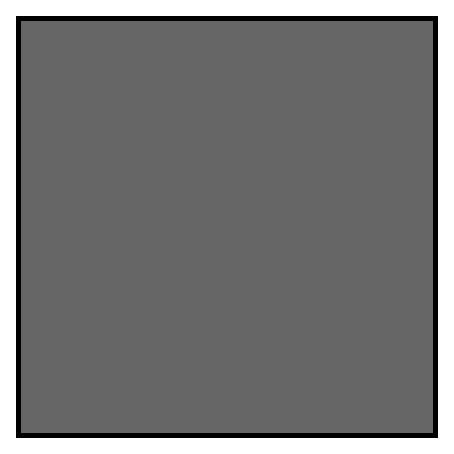
\includegraphics{example.eps}
%% figure caption is below the figure
%\caption{Figure1}
%\label{fig:1}       % Give a unique label
%\end{figure}
%%
%% For two-column wide figures use
%\begin{figure*}
%% Use the relevant command to insert your figure file.
%% For example, with the graphicx package use
%  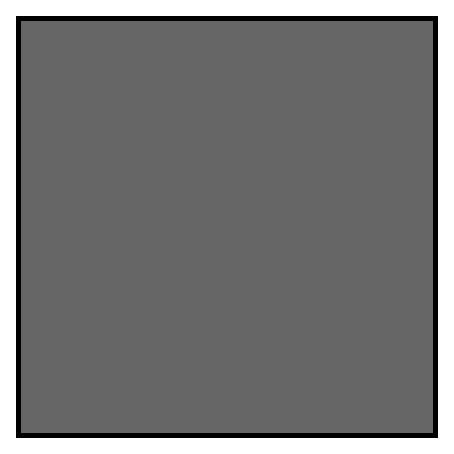
\includegraphics[width=0.75\textwidth]{example.eps}
%% figure caption is below the figure
%\caption{Figure2}
%\label{fig:2}       % Give a unique label
%\end{figure*}
%%
%% For tables use
%\begin{table}[h!]
%% table caption is above the table
%\caption{Please write your table caption here}
%\label{tab:1}       % Give a unique label
%% For LaTeX tables use
%\begin{tabular}{lll}
%\hline\noalign{\smallskip}
%first & second & third  \\
%\noalign{\smallskip}\hline\noalign{\smallskip}
%number & number & number \\
%number & number & number \\
%\noalign{\smallskip}\hline
%\end{tabular}
%\end{table}


\begin{acknowledgements}
If you'd like to thank anyone, place your comments here
and remove the percent signs.
\end{acknowledgements}

% BibTeX users please use one of
\bibliographystyle{spbasic}      % basic style, author-year citations
%\bibliographystyle{spmpsci}      % mathematics and physical sciences
%\bibliographystyle{spphys}       % APS-like style for physics
\bibliography{references}   % name your BibTeX data base

% Non-BibTeX users please use
%\begin{thebibliography}{}
%%
%% and use \bibitem to create references. Consult the Instructions
%% for authors for reference list style.
%%
%\bibitem{RefJ}
%% Format for Journal Reference
%Author, Article title, Journal, Volume, page numbers (year)
%% Format for books
%\bibitem{RefB}
%Author, Book title, page numbers. Publisher, place (year)
%% etc
%\end{thebibliography}

\end{document}
% end of file template.tex

